\subsection{Neutral Transport} \label{sub:NeutralTransport}

Neutrals from gas injection and gas recycling from the wall are:

\begin{itemize}
	\item ionized by interaction with electrons, which produces 
	\begin{itemize}
		\item a plasma ion in the ion particle balance equation \cref{eqn:Continuity} and
		\item an ionization cooling term in the ion energy balance equation \cref{eqn:EnergyIon}; and
	\end{itemize}
%
	\item interacts with a plasma ion to effectively replace a hot ion with a cool ion ( charge exchange cooling term in the ion energy balance equation \cref{eqn:EnergyIon}).
\end{itemize}

The transport of these neutrals are modeled using \acf{TEP} methodology \cite{Stacey1994, Stacey2000a, Stacey2001b, Rubilar2001, Stacey2001c, Mandrekas2003, Zhang2006}. The \ac{TEP} physics are based on a probabilistic description of interacting and transmitting particles within a region of interest (i). The partial current, $J_{ij}$ from a region i (note this is not indicating ions) to region j is described by \cref{eqn:GTneutPartialCurrent}.

\begin{equation}
	J_{ij} = \sum_{k}^{k}J_{ki}T_{0i}^{ku} + \sum_{k}^{i}\left(1-\sum_{l}^{i}T_{0i}^{kl}\right) J_{ki} c_i P_i \Lambda_{ij} + s_i P_i \Lambda{ij}^s
	\label{eqn:GTneutPartialCurrent}
\end{equation}

The first term accounts for all of the partial currents entering region i (see \prettyref{fig:tepschematic}) from all contiguous region k that transmit through region i. This is found by multiplying edge currents, $J_{ki}$ by the transmission probability $T_{0i}^{kj}$. The second term represents all of the partial currents entering region i from contiguous regions that suffer a collision inside of region i. The collision probability is $c_i$, the escape probability is, $P_i$ and the probability that scattered particles from region i escape to region j $\Lambda_{ij}$. The third term represents any internal source, such as recombination. Further description can be found in Section 2 of \citeauthor{Rubilar2001} \cite{Rubilar2001}.


\begin{figure}
	\centering
	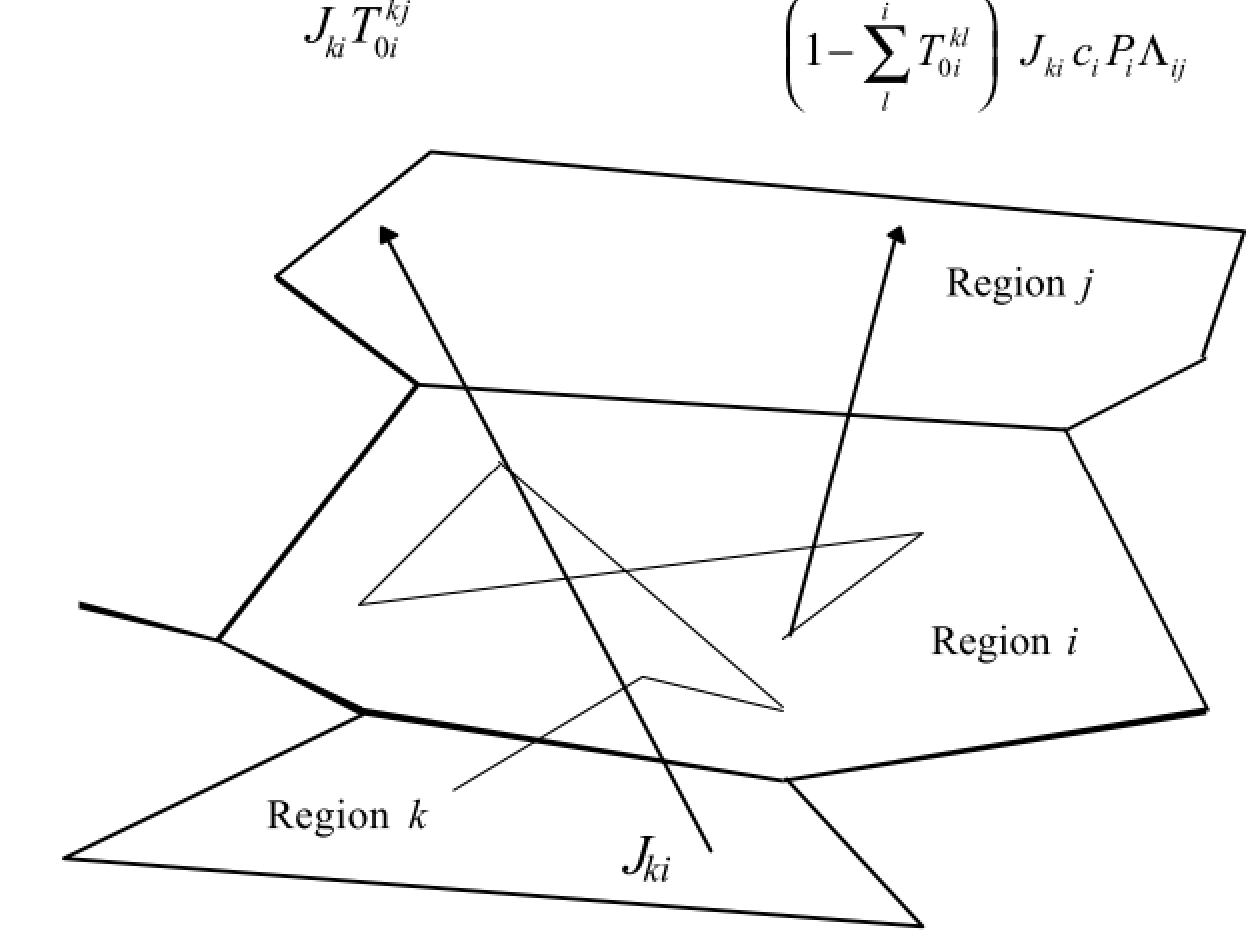
\includegraphics[width=0.7\linewidth]{images/TEP_schematic}
	\caption[TEP]{\acf{TEP} schematic diagram in 2-D geometry \cite{Rubilar2001}}
	\label{fig:tepschematic}
\end{figure}

For our purposes, it has been suggested that a simplified neutral transport implementation from \citeauthor{Stacey2000a} \citeyear{Stacey2000a} \cite{Stacey2000a}, utilizing GTNeut, should suffice. The simplified model breaks the plasma into regions shown in \prettyref{fig:gtneutschematic}. This modeling approach will be utilized initially and modified as needed.

\begin{figure}
	\centering
	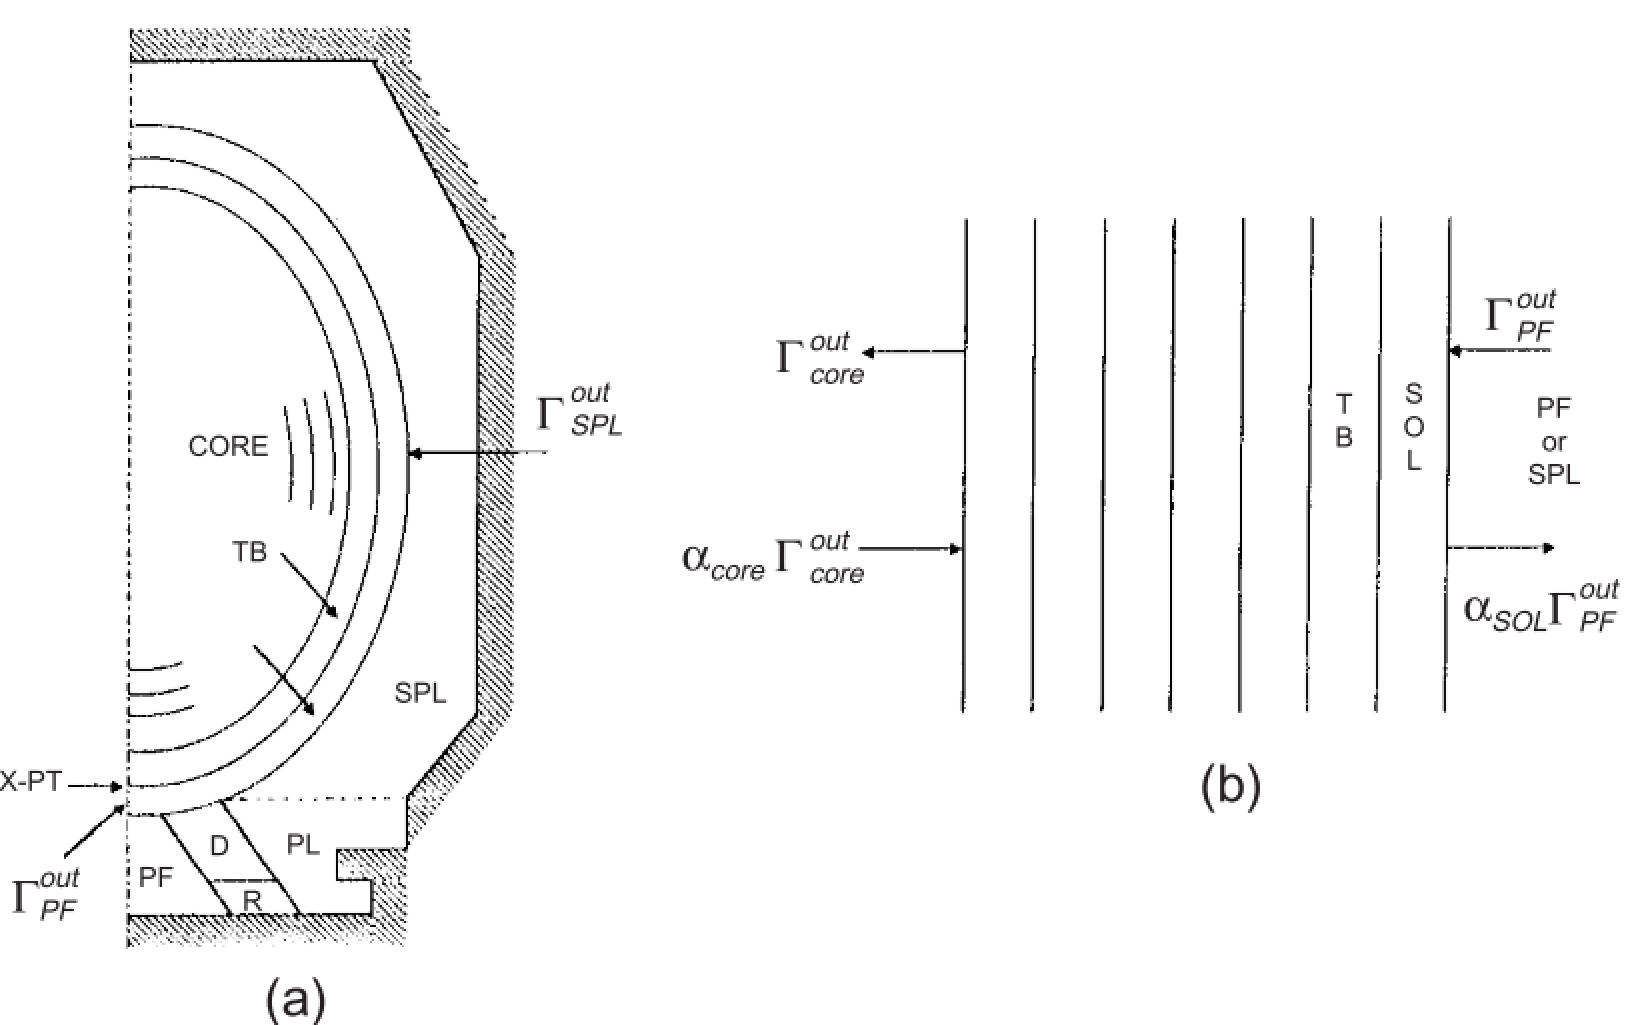
\includegraphics[width=0.7\linewidth]{images/GTNeut_schematic}
	\caption[GTNeutSchematic]{Schematic diagram of the neutral transport model: (a) 2-D TEP model of divertor plasma (D), recycling region (R), private flux (PF), plenum (PL) and SOL plenum (SPL); (b) 1-D ICB model of penetration through SOL and transport barrier (TB) into core. \cite{Stacey2000a}}
	\label{fig:gtneutschematic}
\end{figure}
